\chapter{File Operations}\label{CHAP_FileOperations}

\section{Difficulty: EASY}


\subsubsection*{Exercise 9.E01}

Write a code that generates a file {\code{E09.E01\_HelloWorld.txt}} and write the following
strings to it:
\begin{flushleft}
	{\code{Hello World}}\\
	{\code{Goodbye World}}
\end{flushleft}


\textit{Hints:
You will need the {\code{open()}}, {\code{write()}}, and {\code{close()}} functions. Remember: You can generate new lines by including the string formatter {\code{\textbackslash n}} in the string. To write to a file, use the keyword {\code{w}}.}\\[1cm]

% ------------------------------------------------------------------------------

\subsubsection*{Exercise 9.E02}
Write a code that accepts a food item from the user and appends it to a file called
{\code{E09.E02\_ShoppingList.txt}}. Run your code multiple times to generate a longer
shopping list.\\


\textit{Hints:
You will need the {\code{open()}}, {\code{write()}}, and {\code{close()}} functions. Remember: You can generate new lines by including the string formatter {\code{\textbackslash n}} in the string. To append to a file, use the keyword {\code{a}}.}\\[1cm]

% ------------------------------------------------------------------------------

\subsubsection*{Exercise 9.E03}
Write a code that opens the file {\code{E09.E03\_LotROpeningLine.txt}} and prints the content
to the screen.\\

\textit{Hints:
You will need the {\code{open()}}, {\code{print ()}}, and {\code{close()}} functions. To read from a file, use the keyword {\code{r}}.}\\[1cm]

% ------------------------------------------------------------------------------

\subsubsection*{Exercise 9.E04}
Using a {\code{WHILE loop}}, write all the numbers between 0 and 1,000 into a file called
{\code{E09.E04\_OneThousand.txt}}. Each number should be in a new line.\\


\textit{Hints:
Remember to update the counter inside the {\code{WHILE}} loop and generate new lines using {\code{\textbackslash t}}. Remember to convert numbers into strings using the {\code{str()}} function.}\\[1cm]

% ------------------------------------------------------------------------------

\subsubsection*{Exercise 9.E05}
Write a code that opens the file {\code{E09.E04\_OneThousand.txt}} which you created in
exercise 9.E04. Read in the information in the file and calculate the sum of all numbers
contained.\\

\textit{Hints:
You will need to convert each line into an integer using the {\code{int()}} function.}\\[1cm]

% ------------------------------------------------------------------------------

\subsubsection*{Exercise 9.E06}
Open the file {\code{E09.E06\_PiToOneMillionDigits.txt}} which contains the number $\pi$ to one million digits. Write a code that checks whether your birthday (in the following format {\code{ddmmyyyy}}, for example: {\code{01011960}} for 01.01.2016) is contained in the first million digits of $\pi$.\\


\textit{Hints:
Before you read in the file, have a look at it first using a text editor. Note how the file
contains only one line. Don’t convert either the line or your birthday in a number. Use strings instead.}\\[1cm]

% ------------------------------------------------------------------------------

\subsubsection*{Exercise 9.E07}
Open the file {\code{E09.E07\_PrideAndPrejudice.txt}} (in the public domain and available
from \url{https://www.gutenberg.org}). Read in all the lines in the file and append each to one big string. Then count the number of words in the string and therefore the number of characters in Jane Austen’s Pride and Prejudice.\\


\textit{Hints:
You can add strings to other strings via the {\code{+}} operator. You can count the number of
characters in a string using the {\code{len()}} function.}


% ------------------------------------------------------------------------------

\newpage
\section{Difficulty: MEDIUM}

\subsubsection*{Exercise 9.M01}
Repeat exercise 8.M06 and write a code that asks the user for a city inside an infinite {\code{WHILE}} loop until the user enters the string {\code{STOP}} instead of a new city. This time however, instead of storing the individual user inputs in a list, write them to a file {\code{E09.M01\_Cities.txt}}.\\


\textit{Hints:
Set the loop condition to {\code{TRUE}} to generate an infinite loop. Remember: You can exit a loop prematurely by triggering the {\code{BREAK}} command.}\\[1cm]

% ------------------------------------------------------------------------------

\subsubsection*{Exercise 9.M02}
Some data files will come with comment lines at the top explaining the content of the file.
They usually begin with a {\code{\#}}. It’s always a good idea to check your file before trying to open it so you know exactly what it looks like. If the file includes a comment line, you will want to ignore it while reading in the data.\\
Write a code that opens file {\code{E09.M02\_IrishProvinces.txt}} and prints the Irish provinces stored inside but not the comment line!\\


\textit{Hints:
There are several ways to check whether a line is a comment line. You could check whether
the line includes a {\code{\#}}, you could check whether the first character in the line is equal to {\code{\#}}, or you could use the {\code{startswith()}} string operator.}\\[1cm]

% ------------------------------------------------------------------------------

\subsubsection*{Exercise 9.M03}
Sometimes you get data files that includes empty lines or lines containing nothing but
spaces. If you don’t sort these out, you will end up with a lot of useless overhead in your
data lists.\\
Write a code that opens the file {\code{E09.M03\_USStates.txt}}, extract all the US states in the file and store them in a list called {\code{statesUS}}. Make sure to ignore lines that are empty or contain nothing but strings. Remember to remove the new-line delimiter as well!\\
Once you’re done, display the content of your list and count the number of states.\\


\textit{Hints:
You can remove all spaces from a string using the {\code{strip()}} function. If what remains is an empty string the original string contained nothing but spaces to begin with.}\\[1cm]

% ------------------------------------------------------------------------------

\subsubsection*{Exercise 9.M04}
Write a code that opens the file {\code{E09.M04\_WorldCountryCapitals.txt}}. This file contains two data columns. The first column contains all the countries in the world, the second column
the corresponding capitals. The columns are separated by a tab. Extract the data from the
file and store the countries in a list called countries and the capitals in a list called
capitals. Remember to remove the new line formator {\code{\textbackslash n}} if necessary.\\
Bonus:
Add a routine that asks the user for a country and returns the capital.\\


\textit{Hints:
A tab is represented by {\code{\textbackslash t}} in Python and strings can be split using the {\code{split()}} function. You can remove the last character in a string by putting writing {\code{str = str[:-1]}} at the end.}\\[1cm]

% ------------------------------------------------------------------------------

\subsubsection*{Exercise 9.M05}
Write a code that accepts costumer feedback and stores it in a file called {\code{E09.M05\_Reviews}}. The feedback should include: The name of the costumer, the purchase date, the bought product, and the feedback itself.\\
Bonus: Add another piece of code that accepts a name and returns the feedback given by the costumer.\\

\textit{Hints:
Store the costumer feedback in columns, then use the {\code{split()}} function to separate the data when you read it in.}\\[1cm]

% ------------------------------------------------------------------------------

\subsubsection*{Exercise 9.M06}
Have a look at file {\code{E09.M06\_DeliveryRefernceNumbers.txt}}. The file contains parcel
reference numbers in order of delivery. It is assumed that each delivery takes between 5 and
15 minutes (this includes the drive to the address and the delivery itself). The delivery driver starts work at 9 am.\\
Write a code that accepts a reference number from the user and returns an estimated
delivery time slot. Make sure you can handle invalid delivery references too.\\


\textit{Hints:
You will need to calculate how much time it will take to deliver the parcels before the delivery in question. If all deliveries take five minutes you get the earliest estimate. If all deliveries take 15 minutes you get the latest estimate.}\\[1cm]

% ------------------------------------------------------------------------------

\subsubsection*{Exercise 9.M07}
Have a look at file {\code{E09.M07\_Employees.txt}}. The file contains a list of employees with their name, ID number and birthday. However: Some entries are incomplete and are missing the birthday.\\
Write a code that reads in the data in the file and:
\begin{enumerate}[label=(\alph*)]
	\item stores the name, ID and Birthday of every employee with a complete set of
information in a new file {\code{E09.M07\_EmployeesComplete.txt}}.
	\item stores the names and ID of every employee with a missing birthday in a new file
{\code{E09.M07\_EmployeesMissingBDay.txt}}.
	\item stores the name, ID and birthday of every employee above the age of 65 in a new file
{\code{E09.M07\_EmployeesRetire.txt}}.
	\item accepts a date from the user in the format {\code{dd.mm}} and prints a list of employees whose birthday is on that day with their age in brackets. You can assume all input
dates are valid.
	\item Have a look at the {\code{datetime}} library (\url{https://docs.python.org/2/library/datetime.html}) and write a code that automatically lists all employees with birthdays on the day the code is being executed. You can use the {\code{datetime.date.today()}} function to find today’s date.
	\item You want to send a letter to every employee on their birthday. Generate a loop that
writes a personalised birthday message into a file called {\code{E09.M07\_BDWishes-
[LastName][FirstName].txt}} where {\code{[LastName]}} and {\code{[FirstName]}} are place holders for the last and first name of the employee.
\end{enumerate}


\textit{Hints:
You can solve (a) to (c) inside one big loop.}\\[1cm]

% ------------------------------------------------------------------------------

\subsubsection*{Exercise 9.M08}
Write a code that reads in the DNA sequence stored in {\code{E09.M08\_DNA-Murderer.dat}} and compare it to the suspect's DNA sequences stored in {\code{E09.M08\_DNA-Suspect0000.dat}} to {\code{E09.M08\_DNA-Suspect0050.dat}} to figure out who's the murderer.\\

\textit{Hints:
Use a loop to quickly read in all suspect files. Remember the comparison operator {\code{==}}.}\\[1cm]\\[1cm]

% ------------------------------------------------------------------------------

\subsubsection*{Exercise 9.M09}
The file {\code{E09.M09\_WorldPopulation.txt}} contains the world population from 10,000
years ago until 2015 (source: \url{https://ourworldindata.org/world-population-growth}). The
first line corresponds to the year, the second column to the number of human inhabitants.
Read in the file and determine the year in which the world population surpassed 1 billion
(1,000,000,000).\\

\textit{Hints:
Remember to ignore comment lines and convert strings into numbers before performing
mathematical operations on them.}\\[1cm]

% ------------------------------------------------------------------------------

\subsubsection*{Exercise 9.S01}
Initialize two lists. The first list {\code{numList}} should contain all the numbers between 0 and 1,000. Using the first list, generate a second list {\code{squareNumList}} containing the square roots of all them numbers in {\code{numList}}.\\
Once you have created both lists, create a file called {\code{E09.S01\_SquareRoots.txt}} and
write the content of the lists to it so the file ends up looking like this:
\begin{figure}[H]
		\centering
		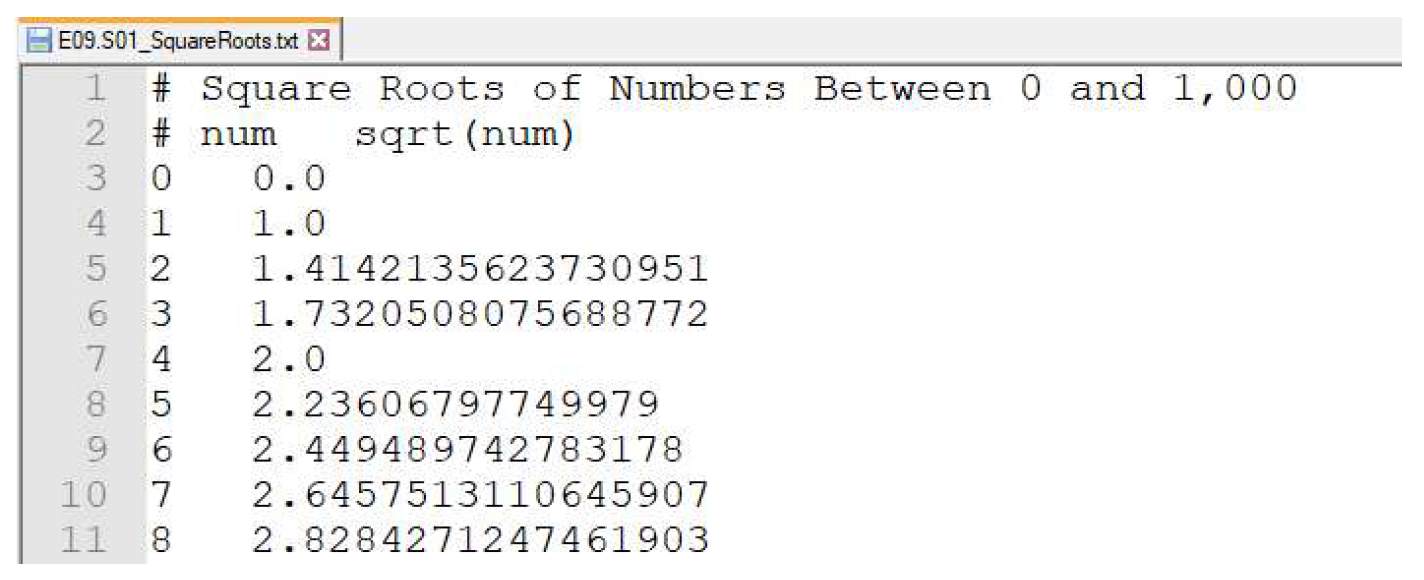
\includegraphics[width=\textwidth]{../IMG/9S01.png} 
\end{figure}

\textit{Hints:
Remember to include \textbackslash n and \textbackslash t to format your output.}\\[1cm]

% ------------------------------------------------------------------------------

\subsubsection*{Exercise 9.S02}
Open the file {\code{E09.S02\_SN2005ek.txt}} which contains spectral data of a supernova
explosion (Source: \url{https://wiserep.weizmann.ac.il/}).\\
Write a code that reads in the information from the file. The first column corresponds to
wavelength, the second column corresponds to flux density. Find the maximum flux and the
corresponding wavelength.\\


\textit{Hints:
You can use the {\code{split()}} function to break down a string into smaller strings which are returned in a list. Remember to convert strings into numbers first using the {\code{float()}} function when you want to perform a mathematical operation on them.}




% ------------------------------------------------------------------------------


\newpage
\section{Difficulty: HARD}

\subsubsection*{Exercise 9.H01}
In this exercise you will be generating a Hangman game.\\
The game works as follows:\\
The computer will choose a word at random. You can then start guessing letters. Once you
have guessed all letters in the word you have won. If the computer finishes drawing the
hangman first, you lose.\\
To write the Hangman game:\\
\begin{enumerate}
	\item Download the file {\code{E09.H01\_sowpods.txt}} (\url{https://github.com/jesstess/Scrabble/blob/master/scrabble/sowpods.txt})into your local working directory. This file contains about 25.000 words commonly used in scrabble.
	\item Read the file and choose one random word and display an output like this:
{\code{"I'm thinking of the following word: \_ \_ \_ \_ \_ \_ \_ \_"}} where the number of underscores is equivalent to the number of letters in the word. To choose a random word, import the {\code{random}} library via {\code{import random}} then generate a random integer between 0 and the length of the list {\code{wordList}} in which you have stored all the words from {\code{E09.H01\_sowpods.txt}}:
{\code{randomNumber = int(random.random() * len(wordList))}}
	\item Prompt the user to guess a letter (you can assume the input is always valid). If the
letter is not in the word, prompt the user to guess again and increase the number of
wrong guesses by one. If the letter is in the word (e.g. the letter a), update the output
like this: {\code{"I'm thinking of the following word: \_ \_ \_ a \_ \_ a \_"}} and prompt the user to guess the next letter.
	\item If the user has guessed the letter before (whether it was correct or not), tell them to guess again but do not increase the number of incorrect guesses.
	\item If the user has guessed the entire word, display it and offer congratulations
	\item Finally, keep track of the number of incorrect guesses. After $x$ (for example $x=11$) incorrect guesses, the user loses the game. Tell the user how many guesses they have
left after each guess.
\end{enumerate}
Bonus:
\begin{enumerate}
	\item Instead of telling the user how many guesses they have left, display a hangman figure after each wrong guess.
	\item Generate a wrapper that runs the game again if the user enters $Y$ after a round and
stops if the user enters $N$
\end{enumerate}

\textit{Hints:
The solutions to this exercise won't include functions since they are not covered in the course these exercises were designed for. It is \textbf{much} easier to solve this exercise with functions, so please use them if you know how to!}






